% \vspace{-2mm}
\section{}
\vspace{-2mm}
    \subsection{CODE}
    \vspace{-2mm}
        \subsubsection{tictoc.cc}
        \label{sec: tictoc.cc code}
            \vspace{-2mm}
            \begin{listing}[h!]
            \inputminted[framerule = 1pt,framesep = 2mm , frame = lines, fontsize=\footnotesize]{c}{./code/week10/Experiment02/tictoc.cpp}
            \vspace{-3mm}
            \caption{\footnotesize experiment 2, tictoc.cc}
            \end{listing}
            \vspace{-6mm}
    \subsection{SIMULATION RESULTS}
    \vspace{-1mm}
    tic/toc의 이름을 갖는 2개의 router 장치로 유선네트워크를 구성한다. tic/toc은 100ms delay를 갖는 유선connection으로 연결이 되어있다.
    Simulation 이 시작하면 tic/toc 이 각각 메세지를 수신했을때 메세지를 서로에게 전송한다.  
    \vspace{-3mm}
        \subsubsection{SCREENSHOT}
        시뮬레이션의 결과에서 2개의 모듈 사이에서 메세지의 전송과 재전송을 잘 담기 위해서 화면녹화 screenshot 영상을 촬영해 youtube에 업로드하였다. 해당 영상은 아래의 링크를 클릭해 이동이 가능하다.
        \vspace{-10mm}
            \begin{center}
                \item \href{https://youtu.be/dQ45SBRxUZ8}
            	{Youtube link of Week10 Experiment 02 Simulation Results Screenshot Video}
            \end{center}
        \vspace{-6mm}
        % 사진 1 2개는 넣어 주자
            \begin{figure}[h!]
            \centering
            \subfloat[Simulation Screenshot 2]{
                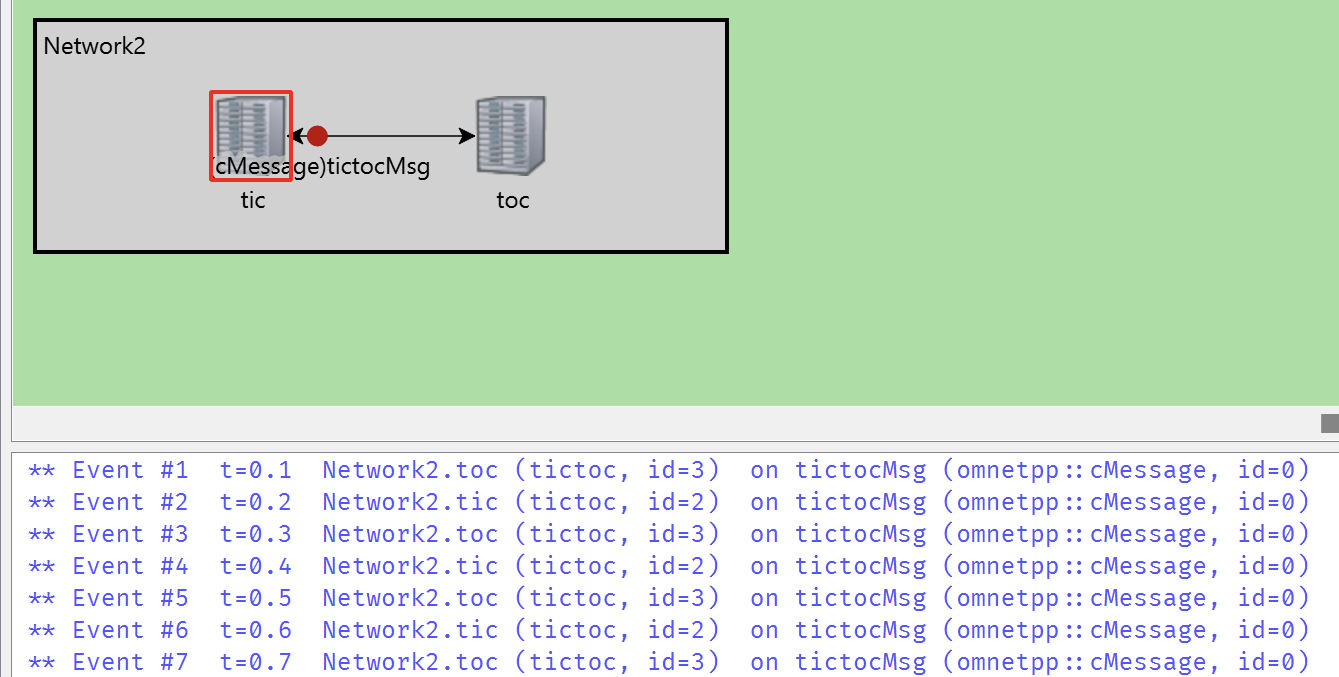
\includegraphics[width=0.47\textwidth]{image/week10/2-1-1.png}
            }\hspace{3mm}
            \subfloat[Simulation Screenshot 2]{
                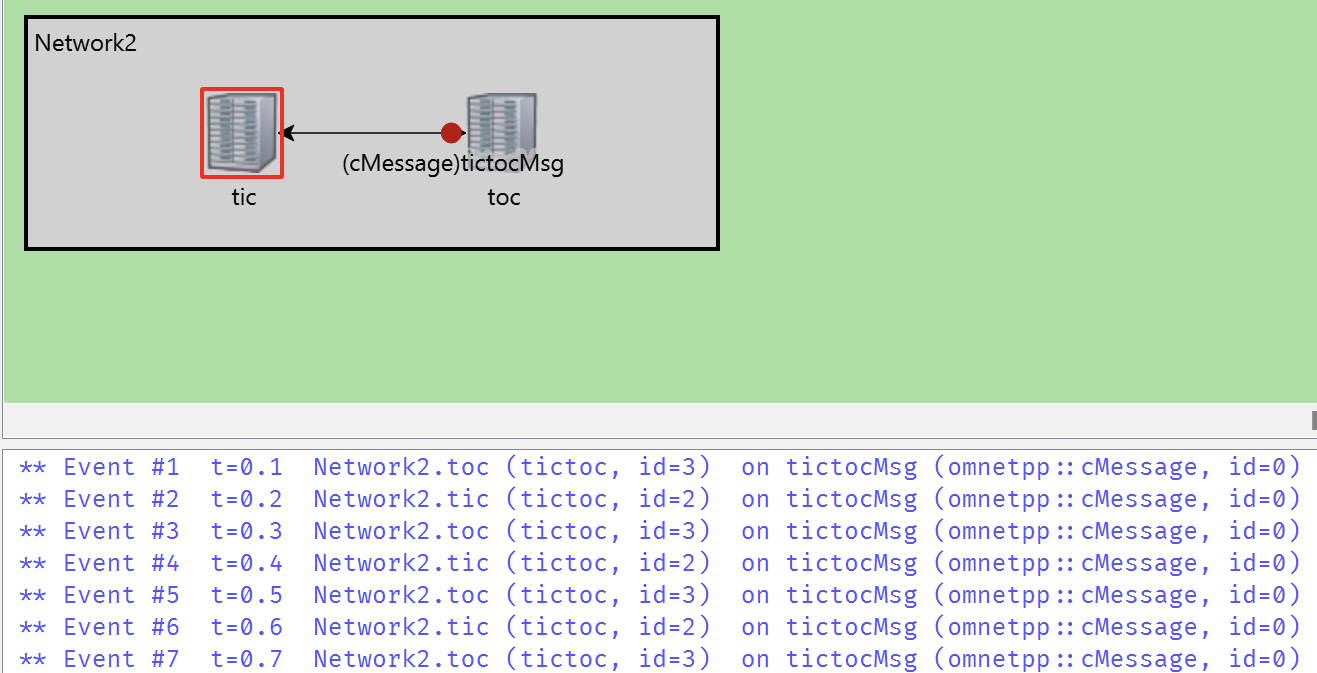
\includegraphics[width=0.47\textwidth]{image/week10/2-1-2.png}
            }
            \caption{Experiment 02 Simulation Results Screenshot}
            \end{figure}
            \vspace{-6mm}
\clearpage
        \subsubsection{RESULTS GRAPH}
        동작을 확인하기 위해서 graph와 함께 Event log를 함께 첨부하였다. \\
            \vspace{-4mm}
            \begin{figure}[!h]\centering 
            	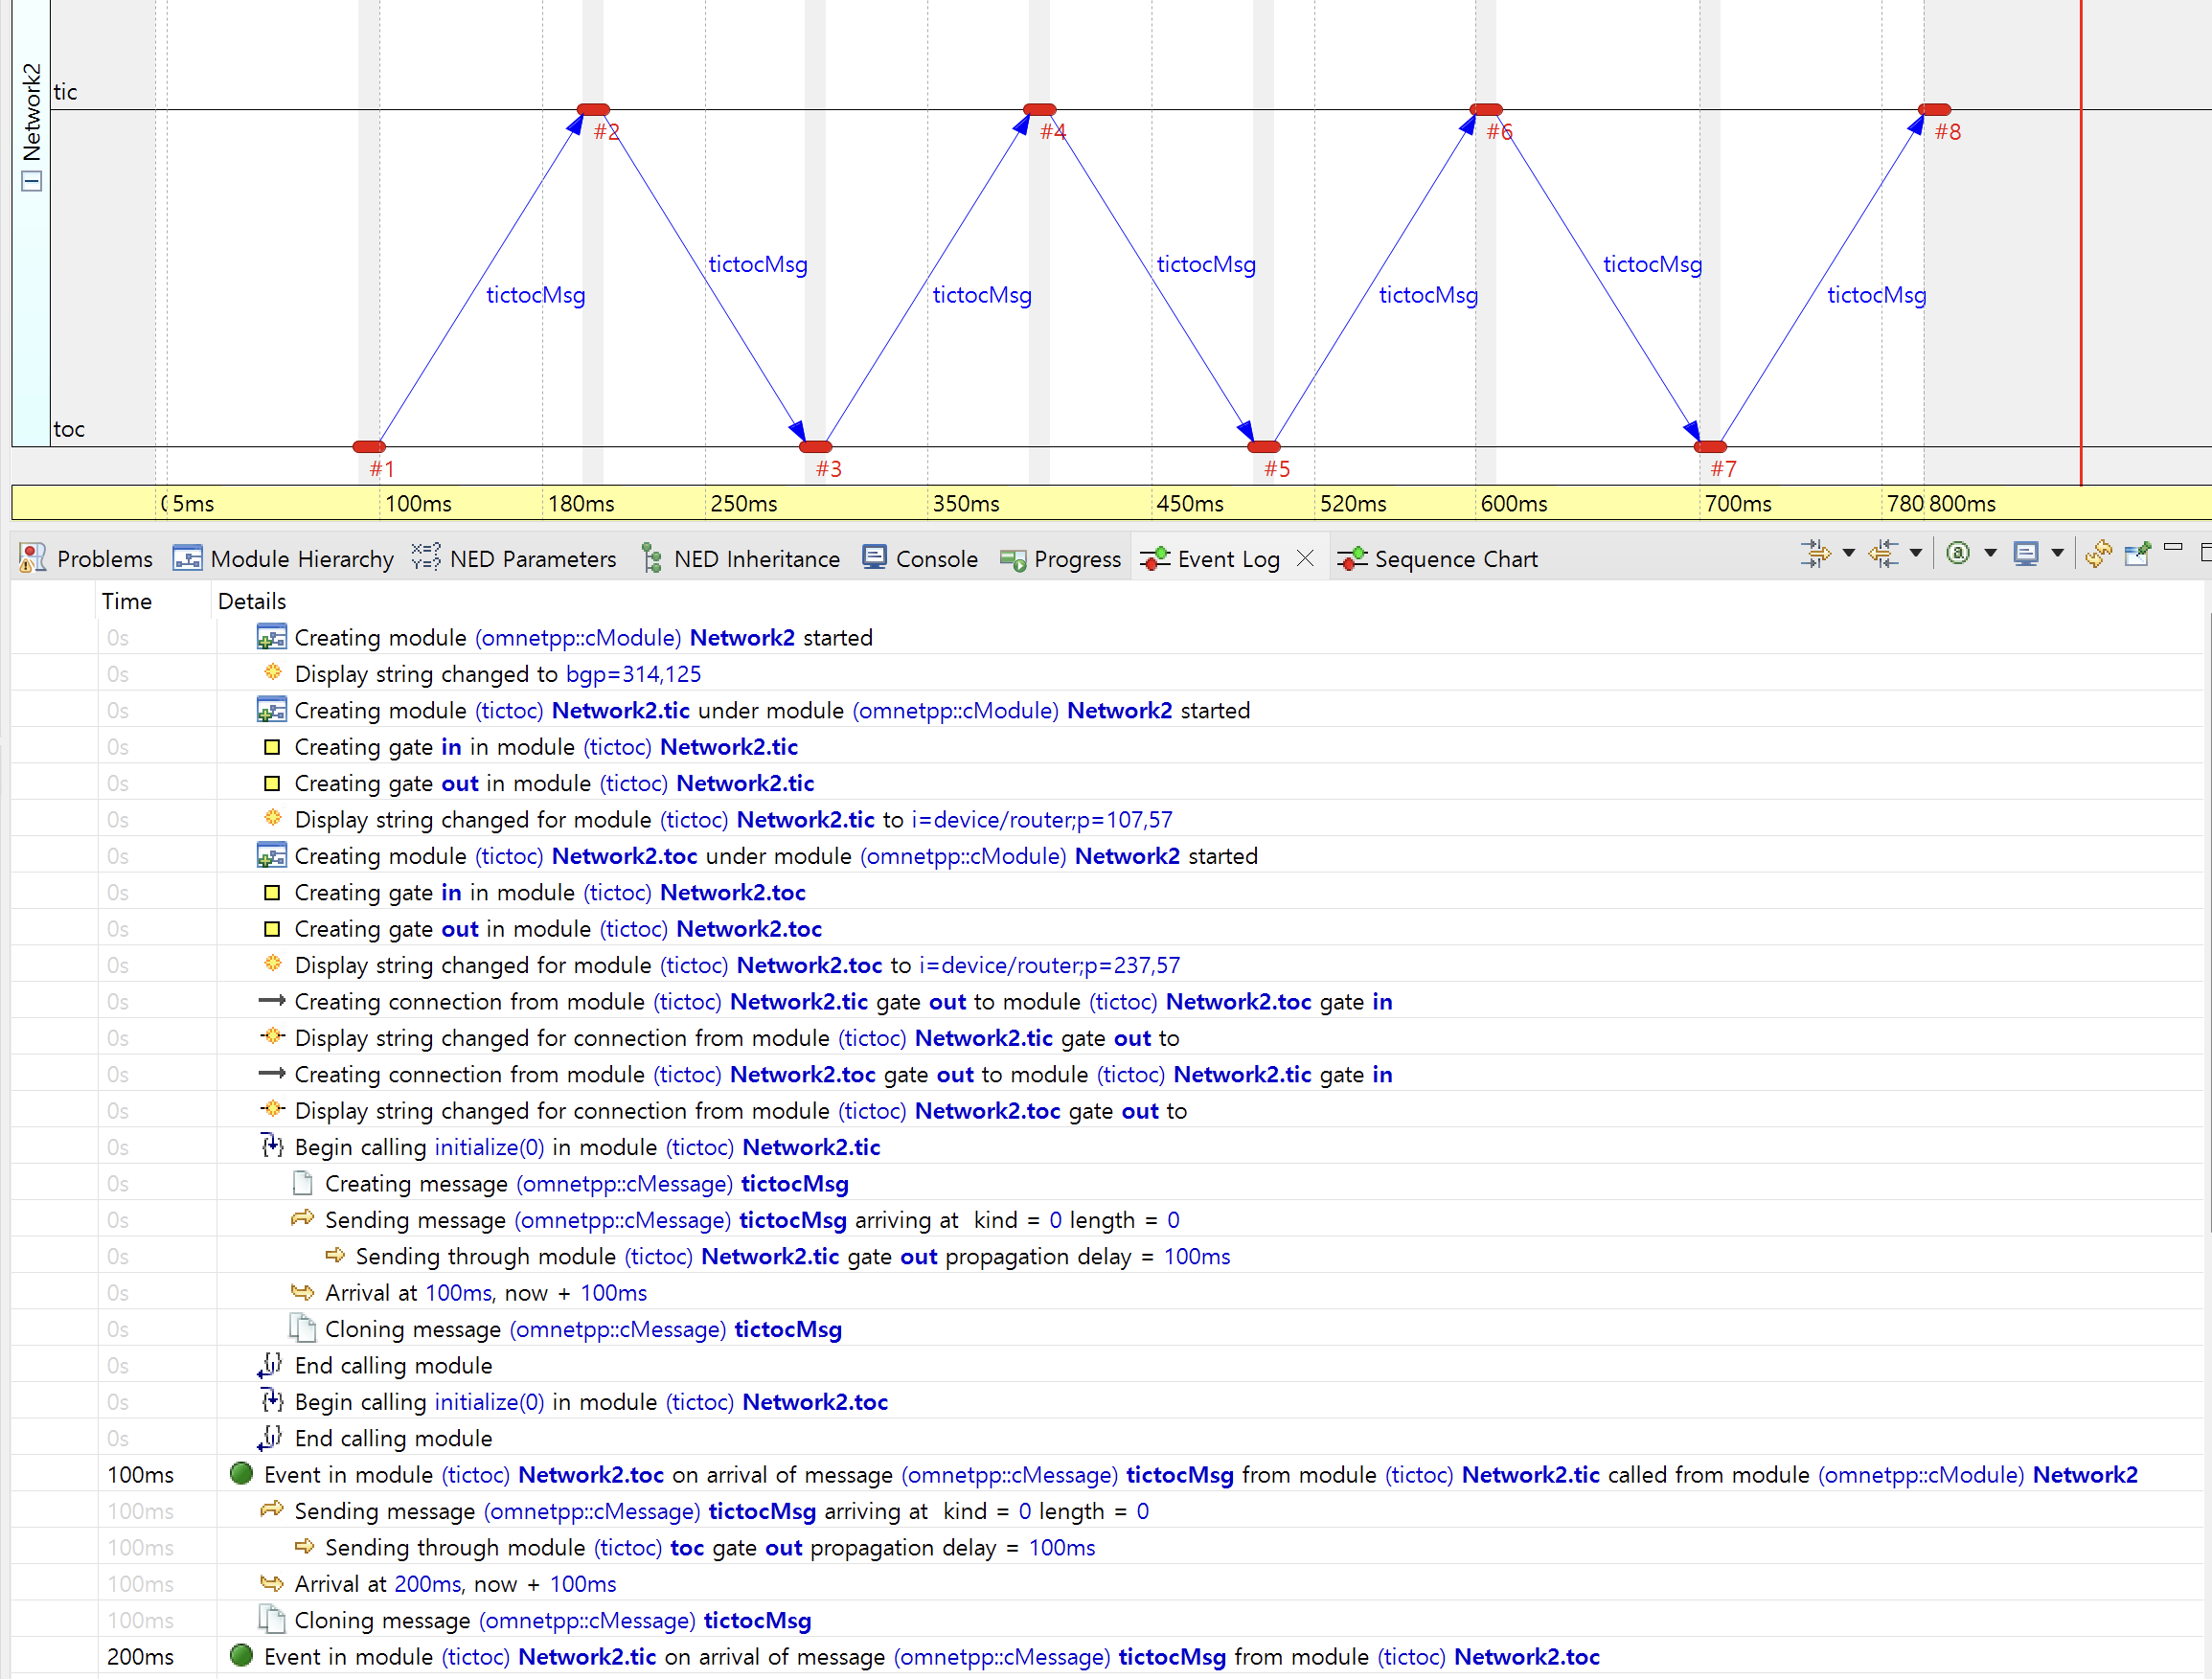
\includegraphics[width=0.99\textwidth]{image/week10/2-2.png}
            	\caption{\footnotesize
            	Experiment 02 Simulation Results Sequence Chart}
            	\vspace{-10pt}
            \end{figure}
            \vspace{-4mm}
        \subsubsection{DISCUSSION}
            \ref{sec: tictoc.cc code} code의 주석에서도 다룬것과 같이 simulation time = 0의 상태에서  module의 이름이 tic일때  “tictocMSG”를 .ned 에서 설정해준 out gate, 즉 tic.out에서 메세지가 보내진다. .ned 파일에서 설정해준 connection에 의해서 channel의 delay와 함께 toc.in 으로 msg가 전송되며 이떄 어떤 module에서 msg를 받았을때의 동작을 정의해 주는 \mintinline{c}{handlemessage()} 에서 parameter로  \mintinline{c}{cMessage *msg} 를 parameter로 받아 수신받은 module에서 수신받은 동일한 msg를 out gate를 통해서 수신하는 동작이 진행된다.
            
            이 과정들을 Graph를 통해서 확인하면 cComponent의 family function인 \mintinline{c}{initialize()} 에서 정의된  msg를 보내는 동작은 tic.out  gate에서 .ned 파일에서 정의해준  connection에 따라 toc.in 의 gate로 전송이 설정해준 100ms의 delay와 함께 주고받는 전송이 되는데 이부분은 위의 chart에서 상위 class에서의 동작이라 별도로 visualize가 되지 않았지만 이동작을 Event log의 기록을 통해서 확인할 수 있었다.
            
            그 후 simulation time t = 100ms 에서, t=0의 앞서 tic.out에서 toc.in의 “tictocMSG” message를 toc module에서 받았기 떄문에 \mintinline{c}{handlemessage} 동작이 toc 에서 이뤄지게 되고, 앞서 설명한 과정과 동일하게 수신받은 message를 tic module로 다시 toc.out에서 tic.in gate로 보내는 동작이 simulation 이 종료될때까지 반복되는 결과를 확인했다.
            
            Experiment 1 과 네트워크 구성방법을 비교해 보았을때, 1에서는 gate를 사용하지 않고 각 모듈을 이름을 지정하여 connection을 cSimple Module의 layer에서 구성해주었는데, 2에서는 이미 namespace가 정의된 tictoc package를 이용하여 cSimplemodule의 subclass 구조를 이용하여 상위클래스에서 module의 connection 과 gate의 structure를 정의해 줌으로서, cSimpleModule에서는 전송하는 동작만 정의해줌으로서, 네트워크 simulation을 효과적으로 구성하는 방법을 확인해볼 수 있었다.
\clearpage